

\begin{document}

\section{Probability Distributions}
A probability distribution describes how the values of a random variable are distributed. 

For example, the collection of all possible outcomes of a sequence of coin tossing is known to follow the binomial distribution, whereas the means of sufficiently large samples of a data population are known to resemble the normal distribution (Central limit Theorem). Since the characteristics of these theoretical distributions are well understood, they can be used to make statistical inferences on the entire data population as a whole.

Recall that probability distributions can be categorised as either \textit{\textbf{discrete}} or \textit{\textbf{continuous}}.
We will look at  
\begin{itemize}
\item how to generate random numbers,
\item how to use probability mass and density functions,
\item how to use cumulative distribution functions,
\item how to determine quantiles.
\end{itemize} 

There is a wide variety of probability distributions available, but we shall only look at a few key distribution. 

\begin{itemize}
\item	The Normal Distribution
\item	The Student $t-$Distribution
\item   The Uniform Distribution
\item	The Exponential Distribution
\item	The Binomial Distribution
\item	The Poisson Distribution
\end{itemize}

If you would like to know what distributions are available you can do a search using the command \texttt{\textbf{help.search("distribution")}}. 

%Here we give details about the commands associated with the normal distribution and briefly mention the commands for other distributions. 
%The functions for different distributions are very similar where the differences are noted.


\subsection{Probability Mass Functions} 

For a discrete distribution, the probability mass function (pmf) is the probability that the discrete random variable $X$ has some specified value (k) i.e. $P(X = k)$. Probability mass functions are determined using the \texttt{\textbf{d}} family of functions. For example, for the binomial distribution, the command is \texttt{\textbf{dbinom()}}, for the Poisson distribution \texttt{\textbf{dpois()}}. 

\subsection{Probability Density Functions} 
For a discrete distribution, the probability density function (pdf) is the relative likelihood that the continuous random variable $X$ will have some specified value (k).
Since for continuous distributions the probability at a single point is zero, it is \textbf{not} equivalent to $P(X = k)$.

Rather the density function is the height of a \textbf{\textit{density curve}} (such as the well-known Gaussian bell-curve) at point $k$.

\begin{center}
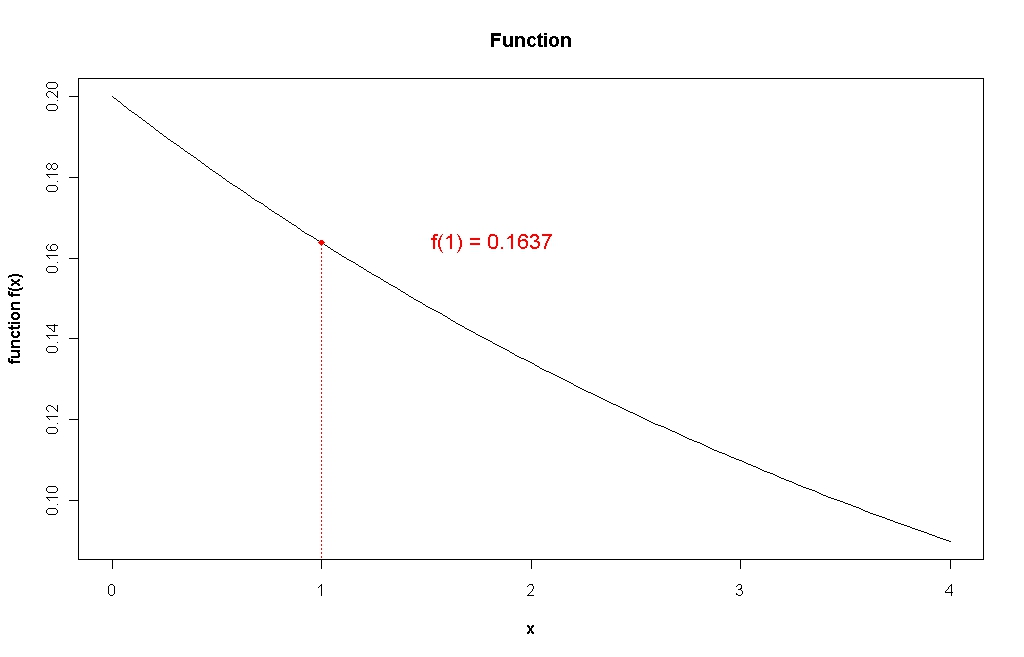
\includegraphics[scale=0.40]{6AFunction}
% \caption{Some function f(x) evaluated at x=1}
\end{center}
 
%\end{document}
 
Probability density functions are determined using the \texttt{\textbf{d}} family of functions. For example, for the normal distribution, the command is \texttt{\textbf{dnorm()}}. 
Necessarily the  \texttt{\textbf{d}} family of functions are more useful for discrete random variables than for continuous variables.

\subsection{Cumulative Distribution Functions}

The cumulative distribution function (cdf) is the probability that the variable takes a value less than or equal to $x$. The cumulative density function is often denoted as $F(x)$.
 
 \[F(x)= P(X \leq x) = \alpha \]

There is little difference in how to treat the cdf for discrete and continuous variables, other than the definition of the complement.
Values for the cumulative distribution functioncan be determined using the \texttt{\textbf{p}} family of functions. 

It is possible to specify the complement probability of the cumulative distribution function (i.e $P(X \geq x)$) directly by additionally specifying the argument \texttt{\textbf{lower=FALSE}}.
 
\subsection{Inverse Cumulative Distribution Functions}

The inverse cumulative distribution function (otherwise known as the quantile function) is a function that yields the quantile $k$ for some specified probability $\alpha$ such that the variable takes a value less than or equal to $k$ with this probability (Recall that $p(X \leq x) = \alpha $).

\[F^{-1}(\alpha) = x  \]

Implementation of the inverse cumulative distribution function requires use of the \texttt{\textbf{q}} family of functions. Quantile functions generally tend to be used with continuous random variables, rather than for discrete random variables.


\section{Continuous Probability Distributions}
In addition to the normal distribution and the $t-$distribution , we will look at two more continuous distribution functions: 
\begin{itemize}
\item The Uniform Distribution
\item The Exponential Distributions
\end{itemize}
\subsection{The Uniform Distribution}

A random variable X is called a continuous uniform random variable over the interval $(a,b)$ if it's probability density function is given by
\[ f_{X}(x) = { 1 \over b-a} \hspace{1cm} \mbox{ when } a \leq x \leq b \mbox{     (otherwise } f_X(x) = 0 ) \]
The corresponding cumulative density function is
\[ F_x(x) = { x-a \over b-a} \hspace{1cm} \mbox{ when } a \leq x \leq b\]


\begin{center}
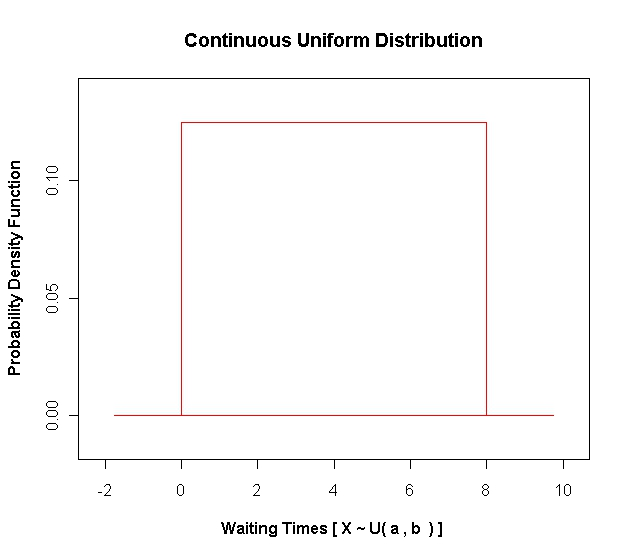
\includegraphics[scale=0.35]{6AUniform}
\end{center}
The continuous distribution is very simple to understand and implement, and is commonly used in computer applications (e.g. computer simulation).
It is known as the `Rectangle Distribution' for obvious reasons. We specify the word ``continuous" so as to distinguish it from it's discrete equivalent: the discrete uniform distribution.
The continuous uniform distribution is characterized by the following parameters

\begin{itemize}
\item The lower limit $a$ (or with \texttt{R}: \texttt{\textbf{min}} )
\item The upper limit $b$ (or with \texttt{R}: \texttt{\textbf{max}} )
\item We denote a uniform random variable $X$ as $X \sim U(a,b)$
\end{itemize}

It is not possible to have an outcome that is lower than $a$ or larger than $b$ ,i.e. $ P(X < a) = P(X > b) = 0$.

We wish to compute the probability of an outcome being within a range of values.We shall call this lower bound of this range $L$ and the upper bound $ U$. Necessarily $L$ and $U$ must be possible outcomes.The probability of $X$ being between $L$ and $U$ is denoted $P( L \leq X \leq U )$.

In the absence of the specified upper and lower limits, the default values of 0 and 1 would be used.

\subsubsection{Generating Random Values}
The most common use of the uniform distribution is the generation of uniformly distributed random variables. The relevant command is \texttt{\textbf{runif()}}. Functions that can be used to manage precision are useful when generating random values.

\begin{verbatim}
> runif(10)
 [1] 0.2558100 0.8738507 0.4521578 0.7868320 0.2310644 0.5265236
 [7] 0.9041761 0.3948904 0.1928505 0.5793142
> runif(10,min=1,max=7)
 [1] 2.822485 4.603547 5.794749 3.766398 2.016349 2.116504 5.863682
 [8] 3.911420 3.434373 6.986899
>
> Another Way of Simulating Dice Rolls
> floor(runif(10,min=1,max=7))
 [1] 1 5 1 6 6 2 1 2 6 3
\end{verbatim}






